\part{泌尿系统疾病急诊}

\chapter{急性肾小球肾炎}

急性肾小球肾炎(acute
glomerulonephritis,AGN)简称急性肾炎,是以急性肾炎综合征为主要临床表现的一组疾病。其特点为急性起病、病程短,患者出现血尿、蛋白尿、水肿、高血压和短暂肾功能损害等。多见于链球菌感染后,故在临床上多称为链球菌感染后肾小球肾炎(poststreptococcal
glomerulonephritis)。少数急性肾炎患者并非由链球菌感染引起的,而是由其他细菌、病毒、原虫等感染引起的,故本病又称急性感染后肾小球肾炎。任何年龄均可发病,但以学龄儿童多见,约占90\%。5~14岁的少年儿童最容易患急性肾炎,男孩患病的机会是女孩的2倍。成人及老年人较少见。冬春季是咽炎、扁桃体炎的好发季节,因此急性肾炎往往发生在这两个季节。

\subsection{病因与发病机制}

\subsubsection{病因}

链球菌感染是最常见的病因,但并非所有链球菌感染都能引起肾炎,只有致肾炎菌株甲族乙型溶血性链球菌致肾炎菌株(β-溶血性链球菌)才能引起本病。呼吸道感染(1、4、12、29、49型等)、皮肤感染(49、55、57、60型)、非链球菌的其他细菌(如葡萄球菌、肺炎双球菌、伤寒杆菌等)、病毒(各型肝炎病毒、麻疹等)、寄生虫(如疟原虫、血吸虫等)和梅毒螺旋体等也可患本病。

\subsubsection{发病机制}

本病主要是由感染所诱发的免疫反应引起,链球菌的致病抗原以前认为是胞壁上的M蛋白,而目前多认为胞浆成分(内链素,endostreptosin)或分泌蛋白(外毒素B及其酶原前体)可能是主要致病抗原,导致免疫反应后可通过循环免疫复合物沉积于肾小球致病,或种植于肾小球的抗原与循环中的特异性抗体相结合形成原位免疫复合物而致病。自身免疫反应也可能参与了发病机制。肾小球内的免疫复合物激活补体,导致肾小球内皮及系膜细胞增生,并可吸引中性粒细胞及单核细胞浸润,导致肾脏病变。

\subsection{诊断}

\subsubsection{临床表现特点}

AGN起病较急,通常于前驱感染(如上呼吸道感染、猩红热、皮肤感染等)后1~3周发病。病情轻重不一,轻者呈亚临床型(仅有尿常规及血清C3异常);典型者呈急性肾炎综合征表现,重症者可发生急性肾衰竭(ARF)。大多预后良好,常可在数月内临床自愈。典型表现有:①尿异常:几乎均有肾小球源性血尿,约30\%患者可有肉眼血尿,常为首发症状和就诊原因。可伴有轻、中度蛋白尿。尿沉渣除红细胞外,早期尚可见白细胞和上皮细胞稍增多,可有颗粒管型和红细胞管型等。②水肿:约80\%的患者出现水肿,轻者为晨起眼睑水肿,严重时波及全身,多为不可凹性水肿,指压无凹痕,但若患者蛋白尿严重,也可出现低蛋白水肿,即为可凹性水肿。③高血压:约80\%患者出现一过性轻、中度高血压(130~150/90~110mmHg),利尿后血压可逐渐恢复正常。少数患者可出现严重高血压,甚至高血压脑病。④肾功能异常:大部分患者起病时尿量减少(常在400~700ml/d),少数甚至少尿(<
400ml/d)。肾功能可一过性受损,表现为轻度氮质血症。多于1~2周后尿量渐增,肾功能于利尿后数日可逐渐恢复正常。仅有极少数患者可表现为ARF,易与急进性肾炎混淆。⑤急性充血性心力衰竭:老年患者发生率较高(可达40\%),儿童患者少见(<
5\%),但在儿童急性左心衰竭可成为急性肾炎的首发症状,如不及时识别,可迅速致死。⑥其他表现:儿童患者常有疲乏、厌食、恶心、呕吐、头痛、腰部钝痛等全身非特异性症状,若感染未控制,患者可表现发热。成人全身症状相对较少。

\subsubsection{实验室检查}

\paragraph{免疫学检查}

绝大多数患者起病初期血中总补体及C3都明显降低,8周内渐恢复正常,对诊断本病意义很大。如血清补体持续降低,可作为病情仍在进展的指标。50\%~80\%患者抗“O”增高,表明近期内曾有链球菌感染,但滴度高低与肾炎的严重程度及预后无关。部分患者起病早期循环免疫复合物(CIC)及血清冷球蛋白可呈阳性。

\paragraph{肾活检}

肾活检的指征为:①少尿一周以上或进行性尿量减少伴肾功能恶化者;②病程超过两个月而无好转趋势者;③急性肾炎综合征伴肾病综合征者。

\subsubsection{诊断注意事项}

于链球菌感染后1~3周发生血尿、蛋白尿、水肿和高血压,甚至少尿及氮质血症等急性肾炎综合征表现,伴血清C3下降,病情于8周内逐渐减轻到完全恢复正常者,即可临床诊断为急性肾炎。如血清抗“O”滴度在1∶400以上,咽拭子培养或皮肤脓液培养找到β溶血型链球菌,有助于判断链球菌感染后肾炎。症状不典型时需多次查尿常规,根据尿的典型改变及补体下降也可作出诊断,但如果病情的发展不象急性肾炎那样经过休息治疗逐渐好转,血清补体C3持续下降超过8周,则应考虑有其他类型肾小球肾炎的可能性,必须作肾穿刺明确诊断。

本病尚应与下列疾病鉴别:

\hypertarget{text00338.htmlux5cux23CHP13-1-2-3-1}{}
(一) 发热性蛋白尿

在某些急性感染发热期间(如扁桃体炎、丹毒、肺炎、骨髓炎等),部分患者往往出现蛋白尿及管型尿,有时镜下血尿,易与不典型急性肾炎相混淆,此可能与肾血流量增加、肾小球通透性增加及肾小管上皮细胞浊肿有关。急性感染期蛋白尿时出现尿的改变发生于感染、高热的极期,不伴高血压及水肿等肾脏疾病的临床表现,热退后尿异常迅速消失。

\hypertarget{text00338.htmlux5cux23CHP13-1-2-3-2}{}
(二) 全身系统性疾病引起急性肾炎综合征

见于系统性红斑狼疮
,过敏性紫癜,结节性多动脉炎或其他弥漫性血管炎等。其中部分患者肾脏受损方面的临床表现与急性肾炎相似,但具有其他系统病变的临床表现及特殊检查所见。

\hypertarget{text00338.htmlux5cux23CHP13-1-2-3-3}{}
(三) 急进性肾炎

少数病例临床起病和典型急性肾炎相似
,但病情急剧恶化,出现进行性肾功能衰竭。凡病程一个月以上,肾功能不好转,反而恶化者,应考虑本病,需及时肾穿刺活检以利早期诊断和治疗。

\hypertarget{text00338.htmlux5cux23CHP13-1-2-3-4}{}
(四) 慢性肾炎急性发作

既往病史不明确的慢性肾炎患者
,若有急性发作时,易与急性肾炎相混淆。除认真询问既往史外,潜伏期短于3~5天,较显著的贫血,血浆蛋白浓度降低,肾功能持续性减退,长期高血压引起心脏和眼底改变,X线平片及B超检查发现双肾已缩小,均有利于慢性肾炎的诊断。

\subsection{治疗}

本病治疗以休息和对症治疗为主。ARF病例应予血液透析,待其自然恢复。AGN为自限性疾病,不宜用糖皮质激素和细胞毒药物。

\subsubsection{休息}

患者一旦发生急性肾炎就应严格卧床休息,直至肉眼血尿消失、利尿消肿、高血压和氮质血症恢复正常,可起床逐步增加活动。一般需要卧床休息2周;其后继续限制活动1~2个月,3个月内避免体力劳动,学生则需要休学。定期检查尿常规,直至完全正常。

\subsubsection{饮食}

发病初期,对饮食成分及液体应有一定限制,以避免加重水肿或肾脏负担。饮食的控制主要根据水肿、高血压及肾功能损害而定。如肾功能正常,蛋白质可不限制,只在氮质血症和明显少尿阶段,蛋白质限在每日每千克体重0.5g,其中高质量蛋白(牛奶、鸡蛋、瘦肉等)占50\%以上。糖类及各种维生素应充分供给。急性期应予低盐(<
3g/d)饮食。在严重水肿或无尿时,则应限制水分摄入。

\subsubsection{治疗感染灶}

一般认为在病灶细菌培养阳性时,应积极应用抗生素治疗,但有些急性肾炎患者在发病前1~3周曾有过呼吸道感染或皮肤感染,发病时炎症已消失,有少数患者根本没有前驱感染病史,对于这些患者病初常规注射青霉素10~14天(过敏者可用大环内酯类抗生素)的必要性现有争议。

急性肾炎是否需要常规摘除扁桃体?笔者主张没有扁桃体炎的患者不需要做扁桃体摘除术。但对反复发作的慢性扁桃体炎则应择期摘除。因为它是β溶血型链球菌栖息场所,是造成急性肾炎迁延不愈和反复发作的重要原因。手术时机选择在扁桃体炎已经得到控制,肾炎已基本稳定(尿蛋白少于+,尿沉渣红细胞少于10个/HP)的时候。手术前后应用青霉素各2周以防止因细菌活跃而导致肾炎复发。

\subsubsection{对症治疗}

包括利尿消肿、降血压,预防心脑并发症的发生。

\paragraph{利尿消肿}

是对症治疗的重点措施。轻、中度水肿者,卧床休息、限制钠盐及水的摄入即可。高度水肿应使用利尿剂。常用噻嗪类利尿剂如氢氯噻嗪,剂量1~2mg/kg,每天1~2次,口服;无效时用袢利尿剂如呋塞米(速尿),40~200mg静注,最大可达400~1000mg/d。应注意如无效,则不应反复使用,因在无尿的情况下,大剂量呋塞米可能引起听力及肾功能的严重损害。

\paragraph{降压}

经休息、控制水盐、利尿等措施而血压仍高者,应给予降压药。首选ACEI或ARB类降压药,如卡托普利12.5~25mg/次口服,每天3次;氯沙坦50~100mg/d口服。

\paragraph{防治心力衰竭}

急性肾炎所致心力衰竭实质上是继发于水、钠潴留高血容量所致的循环充血,与因心肌衰竭的充血性心力衰竭虽症状相似,但病理生理基础不同,故治疗重点应放在限制水、钠摄入,利尿,降压,以矫正水、钠潴留。洋地黄类药物对于急性肾炎合并心力衰竭效果不肯定,不作常规应用,仅于必要时试用。经保守治疗仍难控制的循环充血状态,可用腹膜透析或血液滤过治疗。

\subsubsection{透析治疗}

少数发生ARF者有透析指征时应及时予以透析治疗以帮助患者度过急性期。

\subsubsection{中医药治疗}

\subsection{预后}

急性肾炎是一个自限性疾病,一般预后良好,只要及时去除病因,辅以适当的治疗,在儿童约85\%~90\%,在成人约60\%~75\%可完全恢复。老年人患急性肾炎的机会不多,但其预后在急性肾炎患者中最差。多数病例尿常规改变在3~6个月内恢复,少数患者急性期后临床表现消失,肾功能良好,但尿液中红细胞和少量蛋白可迁延1~2年才逐渐消失。少数病例病程迁延或转为慢性肾炎,个别病例急性期可发生严重并发症而死亡。近年来由于防治工作的改进,死亡率已降至1\%~2\%,甚或无死亡。

\protect\hypertarget{text00339.html}{}{}

\hypertarget{text00339.htmlux5cux23CHP13-1-5}{}
参 考 文 献

1. Schrier RW. Disease of the kidney and urinary tract.
8\textsuperscript{th} ed. Philadelphia:Wolters Kluwer,2007

2. 陆再英,钟南山.内科学.第7版.北京:人民卫生出版社,2008:503

\protect\hypertarget{text00340.html}{}{}

\chapter{急进性肾小球肾炎}

急进性肾小球肾炎(rapidly progressive
glomerulonephritis,RPGN),简称急进性肾炎,是以急性肾炎综合征、肾功能急剧恶化、多在早期出现少尿性ARF为临床特征,病理特征为新月体性肾小球肾炎的一组疾病。

\subsection{病因与发病机制}

\subsubsection{病因}

本病有多种病因,一般将有明确病因的称为继发性急进性肾炎,病因不明者称为原发性(或特发性)急进性肾炎。按病因及发病机制的不同,可将原发性急进性肾炎分为三型(表\ref{tab120-1})。本组疾病大部分病因是继发性的。原发性急进性肾炎只占少部分。现只重点讨论原发性急进性肾炎。

\begin{table}[htbp]
\centering
\caption{急进性肾炎的病因及发病机制分类}
\label{tab120-1}
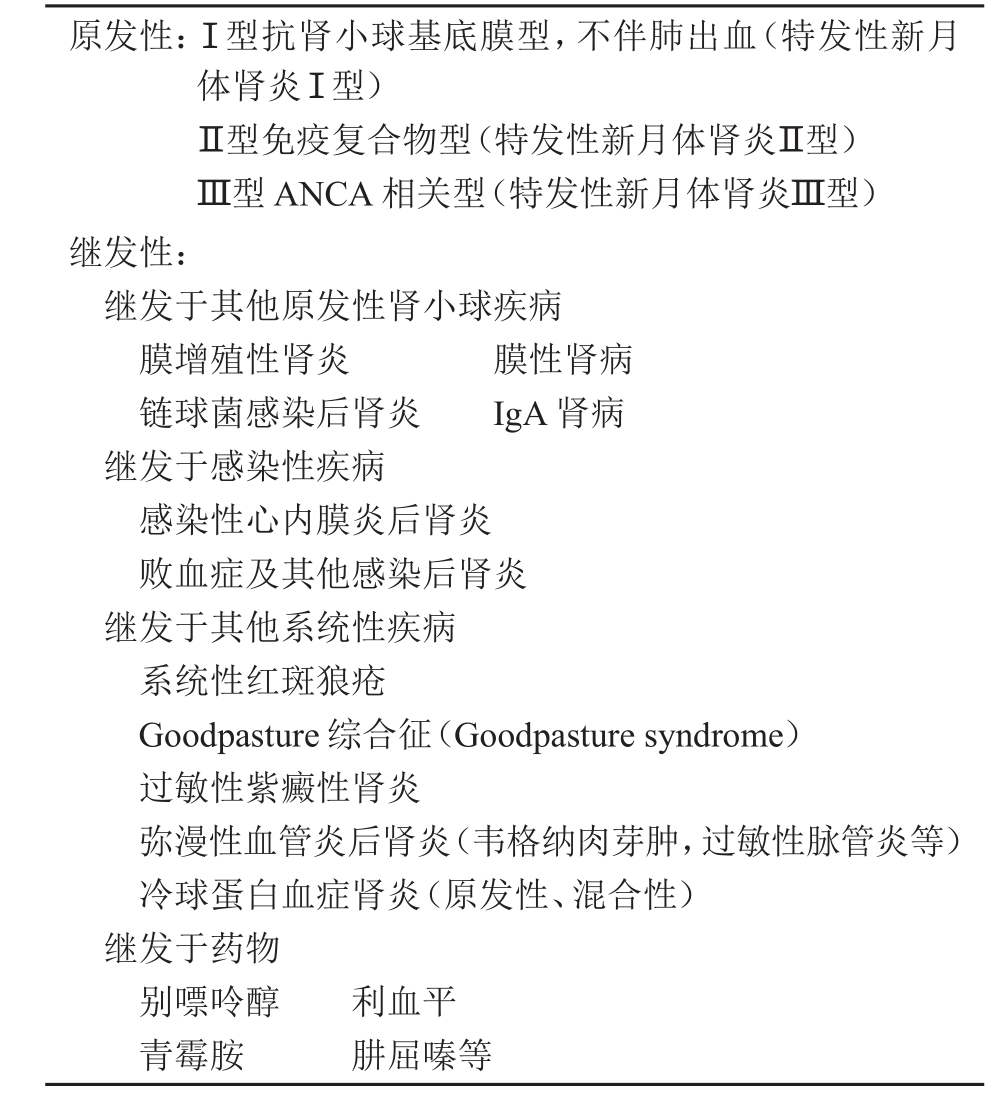
\includegraphics[width=3.33333in,height=3.63542in]{./images/Image00496.jpg}
\end{table}

1996年
Glassok等将免疫荧光病理、血清抗肾抗体和抗中性粒细胞胞浆抗体(ANCA)联合应用于新月体肾炎的分类,将原发性RPGN分为五型:Ⅰ型:抗肾小球基底膜抗体阳性;Ⅱ型:免疫复合物阳性;Ⅲ型:ANCA阳性;Ⅳ型:抗肾小球基底膜抗体和ANCA均阳性;Ⅴ型:寡免疫复合物型,即各种免疫复合物均阴性或很少阳性,抗肾小球基底膜抗体和ANCA亦均阴性。

然而,目前国外权威肾脏病专著仍按上述分为Ⅰ、Ⅱ、Ⅲ型(参见表\ref{tab120-1})。必须指出Ⅱ型RPGN中有一部分ANCA阳性,提示为原发性血管炎造成的新月体肾炎。

\subsubsection{发病机制}

Ⅰ型急进性肾炎的患者血清中可测得抗肾小球基底膜抗体,免疫荧光镜检查在肾小球基底膜上可见线条状均匀一致的IgG沉积,故认为是抗肾小球基底膜抗体介导的病变,又称抗肾抗体型肾炎或原发性急进性肾炎Ⅰ型。此型肾功能损害发展快而重,少尿或无尿的发生率高,预后最差,约占原发性急进性肾炎的20\%。此型患者如伴有肺出血,则称为Goodpasture综合征,属继发性急进性肾炎。

Ⅱ型急进性肾炎患者的血清免疫复合物阳性,而血清抗肾小球基底膜抗体阴性。免疫荧光检查在肾小球基底膜及系膜区有IgG及C3呈不连续的颗粒状沉积,故认为是免疫复合物介导的疾病,又称为原发性急进性肾炎Ⅱ型。本型占原发性急进性肾炎30\%~50\%,预后严重,但较Ⅰ型好。

Ⅲ型患者血清抗肾小球基底膜抗体及免疫复合物均阴性,免疫荧光检查亦无任何沉积物,而血清ANCA阳性,故认为它实际上是以肾脏为主要表现的“小血管炎”,因近年来发现Ⅲ型患者血清抗中性粒细胞胞浆抗体(antineutrophil
cytoplasmic
antibody,简称ANCA)有80\%以上阳性,而Ⅰ型及Ⅱ型则ANCA很少阳性,故Ⅲ型原发性新月体肾炎又称为ANCA相关性原发性新月体肾炎。ANCA是存在于循环中的一种自身抗体,通常在各种血管炎患者的血清中容易测得阳性结果,故认为此型是局限于肾脏的坏死性血管炎。此型约占原发性新月体肾炎的40\%,预后较Ⅰ、Ⅱ型好。

以上分型方法,对了解疾病的发病机制,制订治疗方案和判断预后都具有重要意义。

\subsection{诊断}

\subsubsection{病史与诱因}

RPGN患者约半数以上有上呼吸道感染的前驱病史,其中少数为典型的链球菌感染,其他多为病毒感染。RPGN的诱因包括吸烟、吸毒、接触碳氢化合物等。

\subsubsection{临床表现特点}

除Ⅰ型好发于青、中年外,Ⅱ型及Ⅲ型均以中、老年患者为主。起病较急,病情进展迅速。以急性肾炎综合征(起病急、血尿、蛋白尿、尿少、水肿、高血压),多在早期出现少尿或无尿,进行性肾功能恶化并发展成尿毒症,为其临床特征。患者常伴有中度贫血。恶心、呕吐是常见的消化道症状。部分患者(尤其是Ⅱ型)可因大量蛋白尿导致肾病综合征。Ⅲ型患者常有不明原因的发热、乏力、关节痛或咯血等系统性血管炎的表现。恶心、呕吐是常见的消化道症状。水、钠潴留严重者可发生肺水肿、心包炎、酸中毒、高血钾及其他电解质紊乱,甚至心律失常、脑水肿等严重并发症。

\subsubsection{实验室检查}

\paragraph{尿液检查}

尿蛋白通常阳性,但含量不一,从微量到肾病综合征范围的大量尿蛋白,多为非选择性蛋白尿,变形的多形性红细胞、红细胞管型和白细胞是尿沉渣中常见的有形成分。

\paragraph{肾功能测定}

发病数日或数周后即可发现肾小球滤过率呈进行性下降,内生肌酐清除率下降,血肌酐及尿素氮明显增加,尿比重低且固定。

\paragraph{免疫学检查}

免疫学检查异常主要有抗GBM抗体阳性(Ⅰ型)、ANCA阳性(Ⅲ型)。Ⅱ型患者的血液循环免疫复合物及冷球蛋白可呈阳性,并伴有血清C3降低。

\paragraph{影像学检查}

B超等影像学检查常显示双肾明显增大,有助于区别慢性肾功能不全。

\paragraph{肾活检}

本病确诊需靠肾活检,肾活检光镜检查示>
50\%肾小球有新月体病变诊断可成立。

\subsubsection{诊断注意事项}

凡急性肾炎综合征伴肾功能急剧恶化,无论是否已达到少尿性ARF,应疑及本病并及时进行肾活检。若病理证实为新月体性肾小球肾炎,根据临床和实验室检查能除外系统性疾病,诊断可成立。

原发性急进性肾炎需与以下疾病鉴别:

\paragraph{引起少尿性 ARF的非肾小球病}

包括:①急性肾小管坏死:常有明显的肾缺血(如休克、脱水)或肾毒性药物或肾小管堵塞(如血管内溶血)等诱因,临床上以肾小管损害为主(尿钠增加、低比重尿及低渗透压尿),一般无急性肾炎综合征表现。②急性过敏性间质性肾炎:常有明确的用药史及部分患者有药物过敏反应(低热、皮疹等)、血和尿嗜酸性粒细胞增加等,必要时依靠肾活检确诊。③梗阻性肾病:患者常突发或急骤出现无尿,但无急性肾炎综合征表现,B超等影像学检查可证实尿路梗阻的存在。

\paragraph{肺出血 -肾炎综合征(Goodpasture综合征)}

本病多见于青年人,临床特点是咯血、呼吸困难、血尿及蛋白尿,有时可出现水肿及高血压,迅速出现肾功能衰竭,部分患者在发病前有汽油接触史。多数患者在6个月内死于大咯血所致的窒息或尿毒症。胸部X线摄片可见散在性斑片状或粟粒状阴影。肺及肾组织活检免疫荧光检查均可证实基底膜上有线条状沉积物。

\paragraph{溶血性尿毒症综合征}

多见于婴幼儿,主要临床表现为急性进行性肾功能衰竭、溶血性贫血和血小板减少症三个特点,伴有尿少、无尿、血尿和(或)血红蛋白尿,急性肾功能不全,严重贫血,网织细胞升高,可见到红细胞碎片及芒刺细胞,白细胞总数及中性粒细胞增多,血小板减少及出血倾向。

\paragraph{继发于全身性疾病的急进性肾炎}

如系统性红斑狼疮、过敏性紫癜、结节性多动脉炎、韦格内肉芽肿、进行性系统性硬化症等均可引起继发性急进性肾炎,出现少尿、无尿及肾功能衰竭,如以肾脏起病者,全身症状可不明显或被掩盖,易被误诊。鉴别主要在于提高对原发病的认识,注意全身症状,及早进行有关化验检查以明确诊断。

\paragraph{慢性肾炎急性发作}

慢性肾炎由于某些诱因导致肾功能迅速恶化,由于既往病史不明确,直至感染、劳累、水电解质平衡紊乱等诱因导致肾功能迅速恶化,有时很难与急进性肾炎区别。应用X线平片及B超检查发现双肾已缩小,有利于慢性肾炎的诊断。指甲肌酐数值有助于了解3个月前血肌酐水平。此类患者在诱因纠正后肾功能有部分恢复。

\subsection{治疗}

包括针对急性免疫介导性炎症病变的强化治疗以及针对肾脏病变后果(如钠水潴留、高血压、尿毒症及感染等)的对症治疗两方面。尤其强调在早期作出病因诊断和免疫病理分型的基础上尽快进行强化治疗。

\subsubsection{强化疗法}

\paragraph{强化血浆置换疗法}

应用血浆置换机分离患者的血浆和血细胞,弃去血浆以等量正常人的血浆(或血浆白蛋白)和患者血细胞重新输入体内。开始每日或隔日1次,以后可延至每周3次,每次置换血浆50ml/kg或2~4L,直到血清抗体(如抗GBM抗体、ANCA)或免疫复合物转阴、病情显著改善为止,一般需置换6~10次左右。血浆置换前后必须配合应用糖皮质激素和细胞毒药物,因为致病的蛋白质(如补体、抗体、凝血因子等)被血浆清除后,机体将代偿性增加其合成,故必须用药物抑制。一般常用泼尼松1mg/(kg•d)(2~3个月后渐减)和环磷酰胺2~3mg/(kg•d)(累积量≤8.0g)口服。本疗法适用于各型急进性肾炎,但主要适用于Ⅰ型;对于Goodpasture综合征和原发性小血管炎所致急进性肾炎(Ⅲ型)伴有威胁生命的肺出血作用较为肯定、迅速,应首选。

\paragraph{甲泼尼龙冲击伴环磷酰胺治疗}

为强化治疗之一。具体用法是甲泼尼龙0.5~1g/次或10~15mg/(kg•次)加入5\%葡萄糖液中缓慢静脉滴注,每日或隔日1次,3次为1疗程。必要时间隔3~5天后重复1疗程,一般不超过3个疗程。冲击期间或冲击结束立即改为口服泼尼松(强的松)1mg/(kg•d),+环磷酰胺100~200mg/d,3~6个月后逐渐减量,共用1年左右。近年有人用环磷酰胺冲击疗法(0.8~1g加入5\%葡萄糖液中缓慢静滴,每月1次),替代常规口服。本疗法主要适用于急进性肾炎Ⅱ、Ⅲ型,对Ⅰ型疗效欠佳。甲泼尼龙“冲击”治疗可能出现水钠潴留、诱发感染等副作用,当急进性肾炎已出现少尿、无尿、用呋塞米无效时,应配合透析进行脱水,有感染存在时必须先控制感染。在治疗中密切观察,这些副作用是可以预防或治疗的。

\subsubsection{替代治疗}

凡ARF已达透析指征者应及时透析。对强化治疗无效的晚期病例或肾功能已无法逆转者,则有赖于长期维持透析。肾移植应在病情静止半年(Ⅰ型、Ⅲ型患者血中抗GBM抗体、ANCA需转阴)后进行。

\subsubsection{对症治疗}

对钠水潴留、高血压及感染等需采取相应的治疗措施,参见本书第121章“肾病综合征”治疗部分。

\subsection{预后}

患者若能得到及时明确诊断和早期强化治疗,预后可得到显著改善。早期强化治疗可使部分患者得到缓解,避免或脱离透析,甚至少数患者肾功能得到完全恢复。若诊断不及时,早期未接受强化治疗,患者多于数周至半年内进展至不可逆肾衰竭。影响预后的主要因素有:①疾病的类型:Ⅰ型最差,Ⅱ型次之,Ⅲ型预后较Ⅰ、Ⅱ型好。②临床表现:有前驱感染者疗效较好。病程短,在出现少尿、无尿以前或在肌酐清除率降至10ml/min以前开始治疗疗效较好。③病理指征:组织学已显示出慢性病者(如纤维性新月体、肾小球硬化、间质纤维化及肾小球萎缩)疗效差,但疗效与新月体多少及新月体大小无肯定关系。

\protect\hypertarget{text00341.html}{}{}

\chapter{肾病综合征}

肾病综合征(nephrotic
syndrome,NS)是由多种病因和多种病理类型引起的肾小球疾病中的一组临床综合征,典型临床表现为大量蛋白尿(>
3.5g/d)、低白蛋白血症(血浆白蛋白<
30g/L)、水肿伴或不伴有高脂血症。在肾病综合征中,约75\%为原发性肾小球疾病引起,约25\%由继发性肾小球疾病引起。

\subsection{病因与发病机制}

\subsubsection{病因与临床特征}

NS可分为原发性及继发性两大类,可由多种不同病理类型的肾小球病所引起。引起原发性NS的肾小球病主要病理类型有:

\paragraph{微小病变型肾病}

约占儿童原发性NS的80\%~90\%,成人原发性NS的10\%~20\%。本病男性多于女性,儿童高发。典型的临床表现为NS,仅15\%左右患者伴有镜下血尿,一般无持续性高血压及肾功能减退。约30\%~40\%病例可能在发病后数月内自发缓解,90\%病例对激素治疗敏感,但本病复发率高达60\%。若反复发作或长期大量蛋白尿未得到控制,本病可能转变为系膜增生性肾小球肾炎,进而转变为局灶性节段性肾小球硬化。

\paragraph{系膜增生性肾小球肾炎}

免疫病理检查可将本组疾病分为IgA肾病及非IgA系膜增生性肾小球肾炎。本病在原发性NS中约占30\%,好发于青少年。约50\%患者有前驱感染,可于上呼吸道感染后急性起病,甚至表现为急性肾炎综合征。部分为隐匿起病。本病中,非IgA系膜增生性肾小球肾炎者约50\%患者表现为NS,约70\%伴有血尿,而IgA肾病者几乎均有血尿,约15\%出现NS。

\paragraph{系膜毛细血管性肾小球肾炎}

约占原发性NS的10\%~20\%,好发于青壮年。约1/4~1/3患者常在上呼吸道感染后,表现为急性肾炎综合征。约50\%~60\%患者表现为NS,几乎所有患者均伴有血尿,其中少数为发作性肉眼血尿。肾功能损害、高血压及贫血出现早,病情多持续进展。药物治疗效较差,发病10年后约有50\%的病例将进展至慢性肾衰竭。

\paragraph{膜性肾病}

约占原发性NS的20\%,好发于中老年人。通常起病隐匿,约80\%表现为NS,约30\%伴有镜下血尿,一般无肉眼血尿。约有20\%~35\%患者的临床表现可自发缓解。常在发病5~10年后逐渐出现肾功能损害。本病极易发生血栓栓塞并发症。

\paragraph{局灶性节段性肾小球硬化}

约占原发性NS的5\%~
10\%,好发于青少年男性。多为隐匿起病。约3/4患者伴有血尿,部分可见肉眼血尿。约50\%患者有高血压和约30\%有肾功能减退。

继发性NS的常见病因有过敏性紫癜肾炎(儿童多见)、系统性红斑狼疮肾炎(青少年多见)、糖尿病肾病(中老年人多见)、乙型肝炎病毒相关性肾炎、肾淀粉样变性、骨髓瘤性肾病等。

\subsubsection{病理生理}

\paragraph{大量蛋白尿}

大量蛋白尿是指每日从尿液中丢失蛋白质多达3.5g/1.73m\textsuperscript{2}
,儿童为50mg/kg。大量蛋白尿的产生是由于肾小球滤过膜通透性异常所致。在正常生理情况下,肾小球滤过膜具有分子屏障及电荷屏障作用,当这些屏障作用受损时,致使原尿中蛋白含量增多,当其增多明显超过近曲小管回吸收量时,形成大量蛋白尿。在此基础上,凡增加肾小球内压力及导致高灌注、高滤过的因素(如高血压、高蛋白饮食或大量输注血浆蛋白)均可加重尿蛋白的排出。

\paragraph{低白蛋白血症}

NS时大量白蛋白从尿中丢失,促进白蛋白肝脏代偿性合成增加,同时,由于近端肾小管摄取滤过蛋白增多,也使肾小管分解蛋白增加。当肝脏白蛋白合成增加不足以克服丢失和分解时,则出现低白蛋白血症。此外,NS患者因胃肠道黏膜水肿导致饮食减退、蛋白质摄入不足、吸收不良或丢失,也是加重低白蛋白血症的原因。

\paragraph{水肿}

NS时低白蛋白血症、血浆胶体渗透压下降,使水分从血管腔内进入组织间隙,是造成NS水肿的基本原因。此外,部分患者因有效血容量减少,刺激肾素-血管紧张素-醛固酮活性增加和抗利尿激素分泌增加等,可进一步加重水钠潴留、加重水肿。但近年的研究发现,部分患者血容量正常或增加,血浆肾素水平正常或下降,提示某些原发于肾内钠、水潴留因素在NS水肿发生机制中起一定作用。

肾病性水肿组织间隙蛋白含量低,水肿多从下肢部位开始;而肾炎性水肿(如急性肾炎)组织间隙蛋白含量高,水肿多从眼睑、颜面部开始。肾病性水肿多较明显,与体位有关,严重者常见头枕部凹陷性水肿、全身水肿、两肋部皮下水肿、胸腔和腹腔积液,甚至心包积液等。

\paragraph{高脂血症}

高胆固醇和(或)高甘油三酯血症、血清中LDL、VLDL和脂蛋白(a)浓度增加。其发生机制与肝脏合成脂蛋白增加和脂蛋白分解减弱有关。

\subsection{诊断}

诊断包括以下三个方面:

\paragraph{确诊 NS}

肾病综合征诊断标准是:①尿蛋白大于3.5g/d;②血浆白蛋白低于30g/L;③水肿;④血脂升高。其中①、②两项为诊断所必需。

\paragraph{确认病因}

必须首先除外继发性的病因,才能诊断为原发性NS,最好能进行肾活检,作出病理诊断。原发性NS常见病理类型与临床特征见上述。

\paragraph{判定有无并发症}

①感染:是NS的常见并发症。常见感染部位顺序为呼吸道、泌尿道和皮肤。感染仍是导致NS复发和疗效不佳的主要原因之一。②血栓、栓塞并发症:以肾静脉血栓最为常见(发生率约10\%~50\%,其中3/4病例因慢性血栓形成,临床并无症状),肺血管血栓、下肢静脉、下腔静脉、冠状血管血栓和脑血管血栓也不少见。③急性肾功能衰竭:以微小病变型肾病者居多。④蛋白质及脂肪代谢紊乱。

需要进行鉴别诊断的继发性NS病因主要包括过敏性紫癜肾炎、系统性红斑狼疮肾炎、乙型肝炎病毒相关性肾炎、糖尿病肾病、肾淀粉样变性和骨髓瘤性肾病等。

\subsection{治疗}

\subsubsection{一般治疗}

凡有严重水肿、低蛋白血症者需卧床休息。水肿消失、一般情况好转后,可起床活动。给予正常量0.8~1.0g/
(kg•d)的优质蛋白(富含必需氨基酸的动物蛋白)饮食。由于高蛋白饮食增加肾小球高滤过,可加重蛋白尿并促进肾脏病变进展,故目前一般不再主张应用。水肿时应低盐(<
3g/d)饮食。为减轻高脂血症,应少进富含饱和脂肪酸(动物油脂)的饮食,而多吃富含多聚不饱和脂肪酸(如植物油、鱼油)及富含可溶性纤维(如燕麦、米糠及豆类)的饮食。

\subsubsection{对症治疗}

\paragraph{利尿消肿}

对NS患者利尿治疗的原则是不宜过快过猛,以免造成血容量不足、加重血液高黏倾向,诱发血栓、栓塞并发症。①噻嗪类利尿剂:常用氢氯噻嗪25mg,每日3次口服。长期服用应防止低钾、低钠血症。②潴钾利尿剂:适用于低钾血症的患者。可与噻嗪类利尿剂合用。常用氨苯蝶啶50mg,每日3次,或醛固酮拮抗剂螺内酯20mg,每日3次。③袢利尿剂。常用呋塞米(速尿)20~120mg/d,或布美他尼(丁尿胺)1~5mg/d,分次口服或静脉注射。在渗透性利尿剂应用后随即给药效果更好。④渗透性利尿剂。常用不含钠的右旋糖酐40(低分子右旋糖酐)或羟乙基淀粉(706代血浆)250~500ml静滴,隔日1次。随后加用袢利尿剂可增强利尿效果。但对少尿(尿量<
400ml/d)患者应慎用此类药物,因其易与肾小管分泌的Tamm-Horsfall蛋白和肾小球滤过的白蛋白一起形成管型,阻塞肾小管,并由于其高渗作用导致肾小管上皮细胞变性、坏死,诱发“渗透性肾病”,导致急性肾衰竭。⑤提高血浆胶体渗透压:血浆或白蛋白等静脉输注均可提高血浆胶体渗透压,促进组织中水分回吸收并利尿,如继而用呋塞米60~120mg加于葡萄糖溶液中缓慢静脉滴注,有时能获得良好的利尿效果。但不适当输注大量白蛋白,轻者可延迟疾病缓解,重者可损害肾功能。故仅对严重低蛋白血症、高度水肿而又少尿(尿量<
400ml/d)的NS患者,在必须利尿的情况下方可考虑使用。

\paragraph{减少尿蛋白}

减少尿蛋白可有效延缓肾功能的恶化。常用ACEI如贝那普利10~20mg/次,每日1次;或血管紧张素Ⅱ受体拮抗剂(ARB)如氯沙坦50~100mg/次,每日1次。用ACEI或ARB降尿蛋白时,所用剂量一般应比常规降压剂量大,才能获得良好疗效。

\subsubsection{主要治疗------抑制免疫与炎症反应}

\paragraph{糖皮质激素}

(简称激素)
使用原则和方案一般是:①起始足量:常用药物为泼尼松1mg/(kg•d),口服8周,必要时可延长至12周;②缓慢减药:足量治疗后每2~3周减原用量的10\%,当减至20mg/d左右时症状易反复,应更加缓慢减量;③长期维持:最后以最小有效剂量(10mg/d)再维持半年左右。激素可采用全日量顿服或在维持用药期间两日量隔日一次顿服,以减轻激素的副作用。水肿严重、有肝功能损害或泼尼松疗效不佳时,可更换为甲泼尼龙(等剂量)口服或静脉滴注。根据患者对糖皮质激素的治疗反应,可将其分为“激素敏感型”(用药8~12周内NS缓解)、“激素依赖型”(激素减药到一定程度即复发)和“激素抵抗型”(激素治疗无效)三类,其各自的进一步治疗有所区别。

\paragraph{细胞毒药物}

这类药物可用于“激素依赖型”或“激素抵抗型”的患者,协同激素治疗。若无激素禁忌,一般不作为首选或单独治疗用药。①环磷酰胺:最常用。2mg/
(kg•d)分1~2次口服;或200mg隔日静脉注射。累积量达6~8g后停药。主要副作用为骨髓抑制及中毒性肝损害,并可出现性腺抑制、脱发、胃肠道反应及出血性膀胱炎。②苯丁酸氮芥2mg,每日3次口服,共服用3个月。

\paragraph{环孢素}

作为二线药物用于治疗激素和细胞毒药物无效的难治性NS。常用量为3~5mg/(kg•d),分2次口服。2~3个月后缓慢减量,疗程半年至一年。副作用有肝肾毒性、高血压、高尿酸血症、多毛及牙龈增生等。

\paragraph{吗替麦考酚酯}

作为二线用药,对部分难治性NS有效。常用量为1.5~2g/d,分2次口服,共用3~6个月,减量维持半年。

\subsubsection{个体化治疗方案}

\paragraph{微小病变型肾病}

常对激素治疗敏感,初治者可单用激素治疗。因感染、劳累而短期复发,去除诱因后仍不缓解者可再使用激素,疗效差或反复发作者应使用细胞毒药物,力争达到完全缓解并减少复发。

\paragraph{膜性肾病}

①单用激素无效,必须激素联合烷化剂(常用环磷酰胺、苯丁酸氮芥)。效果不佳的患者可使用小剂量环孢素,一般用药应在半年以上;也可与激素联合应用。②早期膜性肾病疗效相对较好;若肾功能严重恶化,血肌酐>
354μmol/L或肾活检示严重间质纤维化则不应给予上述治疗。③激素联合烷化剂治疗的对象主要为有病变进展高危因素的患者,如严重、持续性NS,肾功能恶化和肾小管间质较重的可逆性病变等,应给予治疗。反之,则提议可先密切观察6个月,控制血压和用ACEI或(和)ARB降尿蛋白,病情无好转再接受激素联合烷化剂治疗。另外,膜性肾病易发生血栓、栓塞并发症,应予以积极防治。

\paragraph{局灶性节段性肾小球硬化}

循证医学表明部分患者(30\%~50\%)激素有效,但显效较慢,建议足量激素治疗{[}1mg/(kg•d){]}应延长至3~4个月;上述足量激素用至6个月后无效,才能称之为激素抵抗。激素效果不佳者可试用环孢素。

\paragraph{系膜毛细血管性肾小球肾炎}

本病疗效差,长期足量激素治疗可延缓部分儿童患者的肾功能恶化。对于成年患者,目前没有激素和细胞毒药物治疗有效的证据。临床研究仅发现口服6~12个月的阿司匹林(325mg/d)和(或)双嘧达莫(50~100mg,每日3次)可以减少尿蛋白,但对延缓肾功能恶化无作用。

\subsubsection{中医药治疗}

单纯中医、中药治疗NS疗效出现较缓慢,一般主张与激素及细胞毒药物联合应用。旨在辨证施治、拮抗激素及细胞毒药物的副作用。雷公藤总苷具有抑制免疫、抑制肾小球系膜细胞增生的作用,并能改善肾小球滤过膜通透性。10~20mg,每日3次口服。主要副作用为性腺抑制、肝功能损害及外周血白细胞减少等,及时停药后可恢复。

\subsubsection{防治并发症}

NS的并发症是影响患者长期预后的重要因素,须积极防治。

\paragraph{感染}

不主张用抗生素预防感染。一旦发现感染,应及时选用对致病菌敏感强效且无肾毒性的抗生素积极治疗,有明确感染灶者应尽快去除。

\paragraph{血栓及栓塞并发症}

当血浆白蛋白低于20g/L时,提示存在高凝状态,即应开始预防性抗凝治疗。可用普通肝素或低分子肝素,或口服华法林。对已发生血栓、栓塞者应尽早用尿激酶或rtPA溶栓治疗。具体用法参见有关章节。

\paragraph{急性肾衰竭}

参见本书第31章“急性肾损伤与急性肾衰竭”。

\paragraph{防治蛋白质与脂肪代谢紊乱}

ACEI及ARB类药物均可减少尿蛋白;中药黄芪(30~60g/d煎服)可促进肝脏白蛋白合成,并可能兼有减轻高脂血症的作用;降脂药物可用洛伐他汀等他汀类药物。NS缓解后高脂血症可自然缓解,则无需再继续药物治疗。

\protect\hypertarget{text00342.html}{}{}

\hypertarget{text00342.htmlux5cux23CHP13-3-4}{}
参 考 文 献

1. 陆再英,钟南山.内科学.第7版.北京:人民卫生出版社,2008:513

2. 张文武.急诊内科手册.北京:人民卫生出版社,2009:533

3. Schrier RW. Disease of the kidney and urinary tract.
8\textsuperscript{th} ed. Philadelphia:Wolters Kluwer,2007

\protect\hypertarget{text00343.html}{}{}

\chapter{急性间质性肾炎}

急性间质性肾炎(acute interstitial
nephritis,AIN)又称急性肾小管-间质肾炎,是一组以肾间质炎细胞浸润及肾小管变性为主要病理表现的急性肾脏病。依病因可分为药物过敏性AIN、感染相关性AIN及病因不明的特发性AIN。本章主要讨论药物过敏性AIN。

\subsection{病因与发病机制}

迄今为止药物仍是AIN最主要的病因,其次是感染,尤其在儿童中。能引起AIN的药物很多,以抗生素、磺胺及非甾体抗炎药(NSAID)最常见。药物(半抗原)与机体组织蛋白(载体)结合,诱发机体超敏反应(包括细胞及体液免疫反应),导致肾小管-间质炎症。由NSAID引起者,还能同时导致肾小球微小病变病。

\subsection{诊断}

\paragraph{近期用药史}

能引起AIN的药物很多,以抗生素、磺胺及非甾体抗炎药(NSAID)最常见。

\paragraph{全身过敏表现}

常见药疹、药物热及外周血嗜酸性粒细胞增多,还可有关节痛或淋巴结肿大。由NSAID引起者全身过敏表现常不明显。

\paragraph{尿异常}

常出现无菌性白细胞尿、血尿及蛋白尿。蛋白尿多为轻度,但由NSAID引起肾小球微小病变病时却可出现大量蛋白尿(>
3.5g/d),乃至肾病综合征。

\paragraph{肾功能损害}

常出现急性肾衰竭,肾小管功能损害出现肾性糖尿、低比重及低渗透压尿。

有上述表现中前两条,再加上后两条中任何一条,即可临床诊断本病。非典型病例(尤其由NSAID致病者)常无第二条,必须依靠肾穿刺活检确诊。

\subsection{治疗}

\paragraph{停用致敏药物}

多数轻症病例即可自行缓解。

\paragraph{免疫抑制治疗}

重症病例宜口服泼尼松30~40mg/d,病情好转后逐渐减量,共服2~3个月。

\paragraph{血液净化治疗}

急性肾衰竭病例应及时行血液净化治疗。

\protect\hypertarget{text00344.html}{}{}

\chapter{溶血性尿毒症综合征}

溶血性尿毒症综合征(hemolytic uremic
syndrome,HUS)是以微血管病性溶血性贫血、血小板减少和肾功能损害三联征为主要表现的一组临床综合征。HUS在成人及儿童均可发病,但典型HUS主要发生于幼儿,起病急骤,它是导致小儿急性肾功能衰竭的重要病因。典型的HUS如能及时诊断,予以正确治疗,多数恢复较好;非典型HUS预后较差,有些进入慢性肾功能衰竭。

HUS广义上可分为典型D\textsuperscript{+} HUS(腹泻相关的HUS,意即“with
diarrhea”,故称为“D\textsuperscript{+}
”)及非典型D\textsuperscript{−} HUS(非腹泻相关的HUS,意即“without
diarrhea”,故称为“D\textsuperscript{−}
”)。按病因又可将HUS分为感染后HUS、遗传性HUS、药物及治疗相关性HUS、继发性HUS及特发性HUS。

典型D\textsuperscript{+}
HUS又称为志贺菌毒素相关性HUS(StxHUS):常与Stx大肠埃希杆菌感染有关,多见于儿童并有急性胃肠炎前驱症状,可有血性腹泻。患者起病急骤,表现为急性溶血性贫血、血小板减少和急性肾功能衰竭,多数患者肾功能可以恢复。

非典型D\textsuperscript{−}
HUS包括各种病因(见下述),但与Stx无关,各年龄均可发病,成人多见,可散发性或家族性发病,患者起病隐匿,无腹泻前驱症状,预后较差,有50\%~60\%患者进入终末期肾病或不可逆性脑损害。

HUS呈全球性分布,各个年龄组均可发病。典型D\textsuperscript{+}
HUS的高发年龄组为6个月~5岁,儿童HUS中90\%为D\textsuperscript{+}
HUS,成人中D\textsuperscript{+}
HUS的比例少于50\%,最高年龄段为50~59岁。Stx大肠埃希杆菌感染后,约38\%~61\%的患者出现出血性结肠炎,有3\%~9\%(散发性感染)和20\%(流行性感染)病例进展至HUS。有报道儿童D\textsuperscript{+}
HUS的年发病率为2.1~10.5/100
000,可呈流行性发病,以大肠埃希杆菌O\textsubscript{157}
∶H\textsubscript{7}
感染的流行(夏秋)季节多见,国外在健康动物(羊、鹿、马、狗、鸟类)的肠道中分离出产毒性大肠埃希菌(VTEC)。有资料提示该病多见于乡村地区,与进食未充分加热的肉制品,不洁的水果、蔬菜、奶制品及饮用污染水有关,在婴儿保育院也有人与人之间传播的报道。

本章主要介绍典型D\textsuperscript{+} HUS。

\subsection{病因与发病机制}

\subsubsection{病因}

HUS的病因与下列因素有关。

\paragraph{感染因素}

感染是诱发HUS的首要因素,大肠杆菌、志贺痢疾杆菌、肺炎链球菌、假单胞菌、伤寒杆菌等细菌以及柯萨奇病毒、埃可(ECHO)病毒、HIV等感染均可诱发HUS。早在1977年,Konowalchuk注意到腹泻患者粪便中分离出来的大肠杆菌可产生一种外毒素,这种毒素对Vero(非洲绿猴)肾细胞具有杀伤作用,在结构和作用上与志贺痢疾杆菌Ⅰ型产生的志贺毒素极为相似,所以称为志贺菌样毒素(Shige-like
toxin,Stx)。1983年Karmali最先提出Stx与HUS的关系,他发现HUS患者多有大肠埃希杆菌(E.coli)感染,这些大肠杆菌均可产生Stx。现在人们普遍认为产生Stx的大肠埃希杆菌(Stx
E.Coli)与儿童典型HUS密切相关,并已从HUS患者分离到多种Stx
E.Coli菌株的血清型:O\textsubscript{111} ∶H\textsubscript{8}
、O\textsubscript{103} ∶H\textsubscript{2} 、O\textsubscript{121}
、O\textsubscript{145} 、O\textsubscript{112} 、O\textsubscript{26}
和O\textsubscript{157} ,其中O\textsubscript{157} ∶H\textsubscript{7}
最易引起严重的出血性结肠炎,导致HUS。北美和西欧的患HUS的儿童中,约90\%可证实曾感染过Stx
E.Coli,其中70\%感染的是大肠埃希杆菌O\textsubscript{157}
∶H\textsubscript{7}
;在印度等发展中国家,也有由志贺痢疾杆菌Ⅰ型引起Stx相关性HUS。

\paragraph{遗传因素}

HUS部分患者有家族性,包括常染色体隐性和显性遗传病例,家族性HUS预后不良,病死率高。

\paragraph{药物及治疗因素}

包括抗排异药物环孢素A(CsA)及他克莫司(FK\textsubscript{506}
),化疗药物如丝裂霉素、长春新碱、阿糖胞苷、柔红霉素等。此外口服避孕药物、抵克立得、奎宁、OKT\textsubscript{3}
,及放射线照射也可诱发HUS。

\paragraph{继发性 HUS}

HUS可继发于系统性红斑狼疮(SLE)、系统性硬化症、抗磷脂抗体综合征、干燥综合征、链球菌感染后肾小球肾炎、膜增殖型肾小球肾炎。某些肿瘤与HUS的发生也有关。妊娠、实体器官(肾、心脏及肝)移植及骨髓移植后也可出现HUS。

\paragraph{特发性 HUS}

病因不明,病变可以复发,有些病例可有补体缺乏。

\subsubsection{发病机制}

1.Stx大肠埃希菌株(如O\textsubscript{157} ∶H\textsubscript{7}
)感染及Stx的细胞毒作用
Stx导致微血管内皮损伤是引起典型D\textsuperscript{+}
HUS的主要因素。Stx可分为两类,即Stx1和Stx2,O\textsubscript{157}
∶H\textsubscript{7}
大肠杆菌可产生Stx1和Stx2或只产生Stx2。流行病学研究发现,由Stx1大肠杆菌引起的出血性肠炎的患儿均不发生HUS,因此HUS主要由Stx2所致。Stx(70kDa)含有一个A亚单位(32kDa)及5个B亚单位(7.7kDa),A亚单位具有生物活性,而B亚单位可以和细胞表面特异的糖脂受体Gb3结合。Stx1和Gb3结合后又很快分离,而Stx2和细胞上Gb3结合时间长。动物试验表明,Gb3受体在体内的分布决定了微血管病变的部位,而细胞表面Gb3受体密度又决定了该细胞对Stx的易感性。Gb3受体在人肾皮质、髓质和肾小管上皮上均有表达,尤以肾小球内皮细胞表面的Gb3受体数目为多,这使得肾小球内皮细胞易受Stx的侵袭。Stx受体的表达范围决定了微血管内皮损伤的区域。

Stx的作用机制:B亚单位先与细胞表面的受体结合后,A亚单位随之分离出来并进入细胞内,通过高尔基复合体和内质网后,直接抑制细胞内蛋白质合成,Stx1和Stx2还可引起内皮细胞凋亡。Stx大肠杆菌和志贺痢疾杆菌感染人体后,与肠黏膜细胞结合及增殖,引起细胞脱落、坏死,临床上出现腹泻;Stx损害肠黏膜血管,引起出血性结肠炎。Stx进入血液循环,到达肾脏,通过Gb3受体介导的细胞摄取作用,Stx进入内皮细胞,A亚单位抑制蛋白质的合成,导致靶细胞死亡。

2.内毒素 、细胞因子及炎性因子参与内皮细胞的损伤
细菌内毒素(LPS)以及一些细胞因子(TNF-α、IL-1等)、化学趋化因子(IL-8、MCP-1)均可以增强Stx的细胞毒作用。尤其是LPS,本身就有损伤内皮细胞的作用,还可以刺激内皮细胞表达内皮细胞黏附分子(P-selectin、ICAM-1),从而增加粒细胞等炎性细胞对内皮细胞的吸附作用。HUS患者常并存有内毒素血症,表明血管内皮损伤可能是内毒素与Stx累加的毒性作用结果。Stx在细胞因子及炎性因子的协同下能够增强中性粒细胞对内皮细胞(特别是肾小球毛细血管内皮细胞)的黏附作用,从而使中性粒细胞激活、数目增加,并释放弹性蛋白酶、NO等加剧内皮损伤,微血栓形成。

3.血小板激活 、内皮损伤与HUS
内皮细胞在维持血管内凝血/纤溶状态平衡中起重要作用,生理条件下的内皮细胞膜及血小板均带有负电荷,两者相互排斥,内皮细胞还能合成并分泌一些抗凝物质,如前列环素(PGI\textsubscript{2}
)、凡登白因子(vWF)等。内皮损伤时,PGI\textsubscript{2}
浓度增加以抑制血小板聚集,减少血栓形成,在HUS患者血液中PGI\textsubscript{2}
的含量明显低于正常,PGI\textsubscript{2}
对血小板的抑制作用被削弱,有利于血小板聚集和血栓形成。

vWF是FⅧ的载体蛋白,由内皮细胞产生,具有介导血小板黏附于血管壁的功能,正常情况下,vWF不进入血液循环,而存在于内皮细胞的Weiber-Palade小体内,内皮细胞损伤后才会释放入外周血中。有证据表明HUS患者急性期血浆中完整的vWF亚基大量减少,vWF的异常结构片段增加,而vWF巨大多聚体则减少。因此,vWF在HUS的发病机制中起很重要的作用,它和血小板上的受体结合,激活血小板,从而促进微血管内血栓的形成。

与内皮损伤密切相关的一氧化氮(NO)在HUS中也起重要的作用,NO由L-精氨酸经NO合成酶催化生成,具有多种生物活性。HUS患者血管内皮损伤时,会引起血流切应力的改变,后者通过改变vWF对蛋白分解酶的敏感性而影响vWF的量;血流切应力的改变还可使内皮细胞NO生成增加,NO对内皮细胞可产生毒性作用并影响邻近细胞,使之释放TNF-α和IL-1,促使白细胞激活,活化的白细胞产生氧自由基与NO相互作用生成毒性极强的过氧亚硝酸根及羟自由基,进一步加重细胞及组织的损伤。血管内皮损伤还可致血管内皮生长因子(vascular
endothelial growth
factor,VEGF)产生增加,HUS患者急性期血清VEGF水平常升高,VEGF促进肾脏微血管再生、修复并有保护血管内皮功能,VEGF水平升高可能有助于减轻肾小球及肾小管损伤。

总之,血小板的激活和血管内皮细胞受损是HUS发病的重要机制。血管内皮损伤可激活血小板,血小板的聚集又能加重内皮的损伤,导致微血管血栓性病变,并继发红细胞机械性损伤而发生溶血,血小板过度消耗而出现低血小板血症和出血,血栓阻塞血流而导致器官缺血性损伤,最终导致HUS的一系列临床表现。

\subsection{诊断}

\subsubsection{临床表现特点}

\paragraph{消化系统}

初期常表现为腹泻,从肠道感染到腹泻的间歇期平均为3天(1~8天),常伴有腹痛、呕吐(30\%~60\%)、发热(30\%),70\%的病例呈出血性结肠炎,大便为黏液性或血性,症状持续1~2周,经短暂的无症状期,随后出现典型的HUS三联征。大便培养有时可发现Stx大肠杆菌,血清学实验针对Stx及O\textsubscript{157}
LPS的抗体阳性可明确诊断。

StxHUS的消化系统表现要与阑尾炎、肠套叠等急腹症鉴别。另外患者还可有肝大,血清转氨酶、淀粉酶、脂酶和血糖水平均可升高,提示肝脏、胰腺功能受损,蛋白丢失性肠病可致低蛋白血症。严重病例还可出现肠黏膜下血管栓塞、假膜形成及肠坏疽。

\paragraph{肾脏}

急性肾衰为本病的突出表现,半数病例为少尿型急性肾衰,水钠潴留引起水肿、心衰,60\%的病例出现高血压,国外50\%患者需透析治疗。尿液检查可有1~2g/d的蛋白尿(偶有肾病综合征),镜下血尿、管型尿,偶有肉眼血尿,重度溶血可有血红蛋白尿。血尿素氮、肌酐升高。溶血、肾小球滤过率下降及代谢性酸中毒可引起高钾血症,同时可有低钠、低钙及继发性高尿酸血症。

病理检查肾脏主要受累部位是肾小球毛细血管袢及肾小动脉。光镜下肾小球病变呈局灶性分布,肾小球毛细血管内皮细胞肿胀,内皮细胞下间隙增宽,结果使毛细血管壁增厚,管腔狭窄,可有微血栓形成,可见纤维样物质及脂质在内皮细胞下聚集。肾小球内系膜区增宽,可见中性粒细胞,偶有新月体形成及坏死表现,肾小球也可呈分叶状。病变的肾小动脉可见内膜下细胞浸润,管壁增厚、坏死,血管腔内血栓形成及管腔闭塞,进而引起局灶或广泛的肾内质坏死。有些病例可有急性肾小管坏死及小管间质病变的表现。免疫荧光可见纤维蛋白、纤维连接蛋白、IgM、C3沿肾小球毛细血管袢、系膜、内皮下及血管壁沉积。电镜下可见内皮细胞肿胀、脱落、内皮细胞下间隙可见颗粒状电子致密物沉积。

典型儿童D\textsuperscript{+}
HUS患者以肾小球受累为主,成人患者病变主要位于动脉和小动脉,伴肾小球缺血及肾小球毛细血管袢皱缩。肾小球病变为主的患者预后较好,而动脉受累严重的患者预后较差。

\paragraph{血液系统}

急性期即有溶血性贫血和血小板减少,血红蛋白短期内降至80~100g/L,但也可低于50g/L。溶血的严重程度与肾衰并不平行,病变最初几周溶血可反复出现。由于微血管病变和过氧化物损伤,末梢血中出现红细胞碎片、棘细胞等异形红细胞。网织红细胞、乳酸脱氢酶及非结合胆红素增加,Coom'b试验常常阴性,急性期可有白细胞升高。由于血小板凝聚、活化、半衰期缩短及破坏增加,致外周血血小板计数减少(通常为30
× 10\textsuperscript{9} /L~100 × 10\textsuperscript{9}
/L),不成熟的血小板增加。血小板功能检查可见血小板聚集功能下降、血小板内β-血小板球蛋白、血小板因子4及血清素水平下降;但血清β-血小板球蛋白、血小板因子4及血清素水平增加。凝血功能检查如凝血酶原时间及部分凝血激酶时间通常正常。

\paragraph{神经系统}

25\%患者可有神经系统症状,包括易激惹、失眠、行为异常、共济失调、震颤及眩晕等。约1/3患者出现神经系统功能异常,如局灶或全身性癫痫发作,少数患者伴有轻偏瘫、张力性体位、木僵和昏迷等。这些症状可能与Stx、低钠血症、低钙血症、尿毒症脑病及恶性高血压有关。部分患者尸检可发现有脑水肿及微血栓形成。

\paragraph{循环及呼吸系统}

有些患者出现循环系统病变,如心肌炎、心源性休克、往往与微血栓形成有关,部分患者可有急性呼吸窘迫综合征。

\subsubsection{诊断注意事项}

临床上具备急性微血管性溶血性贫血、血小板减少和急性肾衰三联征,具有腹泻前驱症状即可诊断典型D\textsuperscript{+}
HUS。肾活检可帮助确诊及估计预后,但急性期有血小板减少和出血倾向,不宜行此项检查。HUS和血栓性血小板减少性紫癜(TTP)在临床表现和病因方面有相似之处,同属血栓性微血管病(thrombotic
microangiopathy,TMA),二者组织学上均有肾小动脉和肾小球内血栓形成。临床上,TTP有多系统表现,除上述三联征表现外,还有发热及不同程度的中枢神经系统受累。但发热、神经系统症状在HUS也较常见。有学者认为,HUS和TTP是一个疾病谱的连续性表现,某些CsA相关性及家族性病例同时具有HUS及TTP的表现,单凭临床表现有时很难区分。一般来说,TTP主要见于成人,起病隐匿,极少有前驱症状,神经系统损害的发生率及严重程度均突出于肾脏病变。实验室检查TTP患者可有不正常的vWF多聚体及vWF裂解蛋白酶缺乏,HUS患者血浆中很少有vWF裂解蛋白酶活性的下降。

\subsection{治疗}

1.按急性肾衰处理
,纠正水电解质平衡,脱水患者应适当补液,但应量出为入,避免补液过量导致肺水肿。纠正低钠、低磷、高钾血症及代谢性酸中毒,对于有明显的尿毒症症状或无尿患者应早期行透析或血液滤过治疗。

2.应避免输血小板,除非有活动性出血或外科手术需要;如血红蛋白低于60g/L,可输新鲜的红细胞,应缓慢输血以免诱发或加重高血压。

3.控制高血压,高分解代谢者需给予适当的营养支持。

4.对肠炎无特殊治疗方法,胃肠道休息非常重要。抗生素不能明确改善Stx有关HUS的预后,有些药物(如磺胺)会增加Stx的释放,故推荐当有菌血症时使用抗生素。严重的缺血性肠病和肠穿孔有时需外科手术治疗。

5.随机对照研究提示抗凝、纤溶药物、抗血小板制剂、免疫球蛋白、新鲜冰冻血浆及血浆置换对急性期患者均无确切疗效,目前对于典型HUS的治疗仍以支持及透析疗法为主。

6.遗留有高血压、慢性肾损害的患者可用ACEI药物治疗,有益于降低蛋白尿,保护肾功能。

典型D\textsuperscript{+}
HUS的预后明显好于成人HUS,多数患者在2~3周内完全恢复,再发病例极为罕见。欧洲的一组长期随访资料表明:该病急性期死亡率为9\%,完全缓解率64\%,遗留慢性肾功能不全及高血压者有4\%,终末期肾病者有9\%,留有其他后遗症者有14\%。临床上下列指标提示预后不佳:①肾脏病理损害严重者(如广泛皮质坏死型HUS);②腹泻时间长,程度重;③无尿期长;④起病初期中性粒细胞明显升高;⑤有严重的神经系统损害。

\hypertarget{text00344.htmlux5cux23CHP13-5-4}{}
非典型D\textsuperscript{−} HUS

非典型D\textsuperscript{−}
HUS与Stx大肠埃希杆菌感染无明确关系,发病无季节倾向,患者起病隐匿,无腹泻前驱症状,病变进行性发展,部分患者可有肾病综合征及重度高血压,并逐渐进展至慢性肾功能衰竭。有些患者病变反复发作,预后较差,尿毒症肾移植后部分患者可有HUS复发。非典型D\textsuperscript{−}
HUS患者死亡率、复发率及终末期肾病发生率都明显高于D\textsuperscript{+}
HUS。该型肾脏组织学表现为肾小球缺血、塌陷,肾小动脉内膜增厚,管腔及肾小球内血栓栓塞。

有些家族性和散发性非典型HUS患者有突出的低C3补体血症,研究发现这些患者补体H因子缺乏,由于H因子基因(HF1)突变而导致补体H因子缺乏或功能异常,不能有效地抑制C3bBb复合物形成和辅助Ⅰ因子对C3bBb进行降解等功能,致使补体通过旁路途径过度激活,是部分非Stx相关性HUS的主要原因。在某些诱因,如病毒、细菌毒素或药物等对内皮细胞具有潜在损害作用因素的诱发下,局部血管内皮损伤和血管内血栓形成,后者又促进C3bBb转化酶形成,而启动补体旁路途径,而由于H因子的数量不足或功能异常,补体过度活化而导致HUS。

非典型D\textsuperscript{−}
HUS无特殊治疗,除加强支持、积极控制高血压、早期透析外,可早期试用血浆疗法去除致病因子,并补充缺乏的补体H因子等。非对照性研究发现儿童及成人患者采用血浆置换和血浆输注疗法可改善肾功能不全,并降低发生终末期肾衰的危险,但血浆疗法不应用于肺炎链球菌感染HUS。

\paragraph{肺炎链球菌引起的 HUS}

肺炎链球菌可产生神经氨酸酶,该酶能暴露红细胞、血小板和肾小球内皮细胞表面的T-F抗原,该抗原与血清中的IgM抗体反应,造成血细胞聚集、肾小球损伤和广泛的微血栓形成,诱发HUS。临床上除有肺炎中毒症状外,Coomb's试验可呈阳性,无网织红细胞增加。治疗可应用抗生素或输注洗涤红细胞,禁用血浆疗法,因成人血浆中含抗T-F抗原的IgM抗体,输注后加重血小板聚集和溶血,该病临床表现重,可有呼吸窘迫、神经系统症状,预后不佳。

\paragraph{家族性 HUS}

包括常染色体显性和隐性遗传,隐性遗传多见,多儿童期发病;而显性遗传成人多见。家族性HUS起病隐匿,有报道HF1与家族性HUS有关,这些患者有持续的低C3补体血症,目前无特异治疗方法,复发率高,可试用血浆置换或血浆输注,预后很差。

\paragraph{移植及 CsA相关性HUS}

肾移植患者可发生HUS,部分属复发性,部分为移植肾新发HUS;有些病例与术后服用环孢素A(CsA)及他克莫司(FK\textsubscript{506}
)有关。国外文献报道肾移植受者服用CsA后HUS的发生率为5\%~15\%,服用FK\textsubscript{506}
的发生率为1\%;但国内报道此类病例极少。HUS常发生于术后最初几周血CsA浓度较高时,研究发现CsA可以增加血小板聚集、血栓素A\textsubscript{2}
的产生,高浓度CsA水平还与血栓调理素及vWF水平相关。

\paragraph{妊娠相关性 HUS}

妊娠期HUS常有先兆子痫,除HUS三联征外,可有肝脏受累及凝血异常,出现弥漫性血管内凝血,如及时终止妊娠,病变多可恢复。产后也可以出现HUS,多发生于有神经系统异常、严重肾衰及严重高血压的患者;正常分娩后3个月内也可发生HUS。产后HUS预后不佳,死亡率达50\%~60\%。

\paragraph{化疗药物相关性 HUS}

化疗药物如丝裂霉素可以诱发HUS,发生率为2\%~3\%,HUS的发生与药物的剂量密切相关,剂量小于30mg/m\textsuperscript{2}
时很少发生HUS。丝裂霉素与博莱霉素或顺铂合用诱发HUS的危险性增加,这些患者预后差,初步研究发现蛋白A免疫吸附治疗有效。

\paragraph{HIV感染相关性HUS}

HIV感染可以并发HUS和TTP,文献报道的发病率有上升趋势,多见于男性同性恋及静脉吸毒者。HUS还可是HIV感染的首发症状,患者多个脏器可见微血栓形成,目前缺乏特异治疗,预后极差。

\protect\hypertarget{text00345.html}{}{}

\chapter{急性尿路感染}

尿路感染(urinary tract
infection,UTI)亦简称尿感,是指各种病原微生物在尿路(包括肾脏、肾盂、输尿管、膀胱、尿道及前列腺)中生长、繁殖而引起的尿路感染性疾病。多见于育龄期妇女、老年人、免疫力低下及尿路畸形者。UTI是最常见的感染性疾病,发病率为1\%~2\%,特别是女性,约1/3的女性在65岁前至少有过一次泌尿系统感染。

引起尿路感染的病原体主要为细菌,也可为真菌、病毒、支原体和寄生虫等。因此,根据引起尿路感染的病原体种类可分为细菌性UTI、真菌性UTI及病毒性UTI等,本章主要叙述由细菌感染所引起的UTI。

根据感染部位可分为上尿路感染和下尿路感染。上尿路感染主要指肾盂肾炎(pyelonephritis)、肾脓肿及肾周脓肿;下尿路感染主要指膀胱炎、尿道炎及前列腺炎。急性肾盂肾炎(acute
pyelonephritis,APN)是指致病菌侵犯肾盂及肾实质,引起急性间质性肾炎及肾小管细胞坏死。当存在尿路结构或功能异常时,反复的尿路感染常可导致肾脏萎缩及肾小盏变形,发展为慢性肾盂肾炎(chronic
pyelonephritis,CPN)。肾脓肿及肾周脓肿是严重的急性泌尿系统感染,常发生于:①尿路梗阻;②免疫缺陷;③糖尿病;④败血症,尤其是金黄色葡萄球菌败血症。膀胱炎(cystitis)指感染局限于膀胱的浅表黏膜。

根据临床有无症状可分为有症状UTI和无症状UTI等。还可分为复杂性UTI和非复杂性UTI,这对于UTI的诊断和治疗十分重要,因为两者的治疗和预后有明显的不同。复杂性UTI是在下列情况下出现的UTI:①存在尿路结构异常(如梗阻、多囊肾、结石及保留尿管等);②存在尿路功能异常(如脊髓损伤、糖尿病或多发性硬化引起的神经性膀胱);③肾实质性损害;④系统性疾病导致患者免疫力低下(如糖尿病、艾滋病等)。而非复杂性UTI则无上述情况。

UTI还可分为初发感染(initial infection)和反复感染(recurrent
infection),后者又可分为复发(relapse)和重新感染(reinfection)。复发指治疗后症状消失,尿菌阴转后在6周内再出现菌尿,菌种与上次相同(菌种相同且为同一血清型)。重新感染约占反复感染的80\%,指治疗后症状消失,尿菌阴性,但在停药6周后再次出现真性细菌尿,菌株与上次不同。

菌尿(bacteriuria)指尿中有细菌生长。真性菌尿(significant
bacteriuria)指清洁中段尿培养菌落计数≥10\textsuperscript{5}
,表明为尿路感染而不是采集标本时造成的污染。急性尿道综合征(acute
urethral
syndrome)指有尿频、尿急、尿痛但无真性菌尿。急性尿道综合征中有70\%为尿路感染,常伴有脓尿,一般为沙眼衣原体(多见于生育期女性)、真菌、结核菌等感染,也可能是尿路周围邻近组织的感染;其余30\%无明确的致病微生物,常不伴有脓尿,可能与局部刺激有关。

急性UTI可以是复杂性UTI,也可以是非复杂性UTI;可以是初发感染,也可以是反复感染。某些慢性UTI在其病程的某一阶段也可以急性发作。急性UTI病原体以细菌最常见,是本章讨论的重点。

\subsection{病因与发病机制}

\subsubsection{致病菌}

UTI最常见的致病菌是革兰阴性杆菌,其中以大肠杆菌最常见,约占全部UTI的80\%~90\%,其次为变形杆菌、克雷伯杆菌。近10\%~15\%的UTI还可由革兰阳性菌引起,主要为葡萄球菌属和粪链球菌。约90\%门诊患者和50\%住院患者的病原菌是大肠杆菌,多见于无症状性菌尿、非复杂性UTI和初发UTI。医院内感染、复杂性或复发性UTI、尿路器械检查后发生的UTI,则多为粪链球菌、变形杆菌、克雷伯杆菌和铜绿假单胞菌属所致。其中变形杆菌常见于伴有尿路结石者,铜绿假单胞菌多见于尿路器械检查后,金黄色葡萄球菌则常见于血源性UTI。真菌感染(主要为念珠菌属)多发生于留置尿管、糖尿病、使用广谱抗生素或免疫抑制剂的患者。多种病原体混合感染仅见于长期放置导尿管、尿道异物(结石或肿瘤)、尿潴留伴反复器械检查,以及尿道-阴道(肠道)瘘等患者。

\subsubsection{发病机制}

在生理情况下,尿道口附近可有少量细菌生长,尿道的远端可有少量的葡萄球菌和类白喉杆菌(diphtheroids),而泌尿系统的其他部分则应是无菌的。95\%以上的UTI是上行感染(逆行感染),即寄生于肠道的致病菌首先附着于阴道、尿道口周围和远端尿道的黏膜,并沿尿道逆行至膀胱、输尿管、肾盂,并可通过肾乳头的Belini管上行至集合管系统。肾脏的髓质是易感部位,因为这里的渗透压高,血供少,影响了抗体及吞噬细胞的活力。某些因素如性生活、尿路梗阻、医源性操作、生殖器感染等可导致上行感染的发生。其他感染途径尚有:血道感染:指致病菌通过血运到达肾脏和尿路其他部位引起的感染。少见,不足3\%。多发生于患有慢性疾病或接受免疫抑制剂治疗的患者。直接感染:泌尿系统周围器官、组织发生感染时,病原菌偶可直接侵入到泌尿系统导致感染。淋巴道感染:盆腔和下腹部的器官感染时,病原菌可从淋巴道感染泌尿系统,但罕见。

人体对UTI有一定的防御能力。机体的防御机制包括:①排尿的冲刷作用(washout);②尿道和膀胱黏膜的抗菌能力;③尿液中高浓度尿素、高渗透压和低pH等;④前列腺分泌物中含有的抗菌成分;⑤感染出现后,白细胞很快进入膀胱上皮组织和尿液中,起清除细菌的作用;⑥输尿管膀胱连接处的活瓣,具有防止尿液、细菌进入输尿管的功能。

以下情况为UTI的易感因素:①尿路梗阻:如结石、前列腺增生、狭窄、肿瘤等均可导致尿液积聚,细菌不易被冲洗清除,而在局部大量繁殖引起感染。②膀胱输尿管反流:输尿管壁内段及膀胱开口处的黏膜形成阻止尿液从膀胱输尿管口反流至输尿管的屏障,当其功能或结构异常时可使尿液从膀胱逆流到输尿管,甚至肾盂,导致细菌在局部定植,发生感染。③机体免疫力低下如长期使用免疫抑制剂、糖尿病、长期卧床、严重的慢性病等。④神经源性膀胱:支配膀胱的神经功能障碍,如脊髓损伤、糖尿病、多发性硬化等疾病,因长时间的尿液潴留和(或)应用导尿管引流尿液导致感染。⑤妊娠:约2\%~8\%的妊娠妇女可发生UTI,与孕期输尿管蠕动减弱、暂时性膀胱输尿管活瓣关闭不全及妊娠后期子宫增大致尿液引流不畅有关。⑥性别和性生活:女性尿道较短(约4cm)而宽,距离肛门较近,开口于阴唇下方是女性易发生UTI的重要因素。性生活时可将尿道口周围的细菌挤压于膀胱引起UTI。包茎、包皮过长是男性UTI的诱因。⑦医源性因素:导尿或留置导尿管、膀胱镜或输尿管镜检查、逆行性尿路造影等可致尿路黏膜损伤、将细菌带入尿路,致UTI。⑧泌尿系统结构异常:如肾发育不良、肾盂及输尿管畸形、移植肾、多囊肾等。⑨遗传因素。

并不是所有种类的大肠杆菌属均可以引起UTI,可以引起正常结构与功能的泌尿系统发生UTI的尿路致病大肠杆菌的种类是有限的。但是,当存在尿路梗阻、反流、异物时,非致尿路致病性大肠杆菌也可以引起UTI。人们发现从有症状的UTI的患者尿中培养出的大肠杆菌比从无症状性菌尿的患者尿中培养的大肠杆菌有较多的K(荚膜)抗原和P(菌毛)抗原,有更强的黏附力。因此,不同的致病菌的毒力是不同的。变异杆菌、克雷伯杆菌因其有尿素酶,可以将尿素分解为氨,增加了尿液的碱性,因而不易被清除。

\subsection{诊断}

\subsubsection{临床表现特点}

典型的急性下尿路感染的症状为尿频、尿急、尿痛及排尿不适,尿镜检可以发现白细胞增多,血尿可以是镜下血尿,也可以是肉眼血尿。一般无发热及肾区疼痛。

典型的急性上尿路感染(主要为急性肾盂肾炎)的症状为寒战、高热、腰痛,可以伴尿频、尿急、尿痛及排尿不适等下尿路感染的症状。肾区叩击痛明显,血白细胞计数增高,有血尿及脓尿,尿中可以发现白细胞管型。急性肾盂肾炎起病急,除上述表现外,常有恶心、呕吐,部分患者可有夜尿增多。在复杂性急性肾盂肾炎时常可发生脓毒症,如糖尿病患者可以出现急性肾乳头坏死,脱落的肾乳头阻塞输尿管,常导致严重脓毒症。

但是临床中遇到许多患者症状不典型,很难区分上、下尿路感染。急性肾盂肾炎可以没有发热及肾区疼痛,而下尿路感染可以没有尿频、尿痛及排尿不适等尿路刺激症状。在有下尿路刺激症状并有真性菌尿的患者中只有50\%~70\%感染局限于膀胱,其余30\%~50\%存在隐匿性的上尿路感染。因此在急诊工作中对于单纯表现为下尿路感染的患者也应警惕隐匿性上尿路感染的存在。有时,UTI不表现出任何尿路感染的症状,只有乏力、发热、全身不适等症状,易误诊和漏诊。

\subsubsection{实验室检查}

\paragraph{尿常规检查}

尿液常混浊,可有异味。常规检查可有白细胞尿、血尿、蛋白尿。增多,如发现白细胞管型,有助于肾盂肾炎的诊断。尿蛋白常为阴性或微量。

\paragraph{尿细菌学检查}

UTI诊断的确立,主要依靠尿细菌学检查。①尿沉渣镜检细菌:清洁中段尿的没有染色的沉渣用高倍镜找细菌,检出率达80\%~90\%,可初步确定是杆菌或球菌、是革兰阴性还是革兰阳性细菌,对及时选择有效抗生素有重要参考价值。②尿细菌定量培养:可采用清洁中段尿、导尿及膀胱穿刺尿做细菌培养,中段尿细菌定量培养菌落计数≥10\textsuperscript{5}
/ml,称为真性菌尿,可确诊尿感;10\textsuperscript{4}
~10\textsuperscript{5} /ml为可疑阳性,需复查;如<
10\textsuperscript{4}
/ml,可能为污染。耻骨上膀胱穿刺采集标本培养有菌落生长,即为真性菌尿。

\paragraph{血常规检查}

急性肾盂肾炎时血白细胞常升高,中性粒细胞增多,核左移。

\paragraph{B型超声检查}

B型超声检查可以发现尿路的结构异常,如梗阻、肾盂积水、多囊肾等,应作为儿童和成人UTI的常规检查。

\paragraph{影像学检查}

X线尿路检查包括尿路平片、静脉肾盂造影(IVP)、逆行尿路造影、排尿时的膀胱输尿管造影等,其目的为了解尿路情况,及时发现有无尿路结石、梗阻、反流、畸形等导致UTI反复发作的因素。但应掌握下列适应证:①任何类型的男性UTI;②儿童,尤其是年龄<
5岁的儿童UTI;③对于初次发生的女性UTI原则上不做X线尿路检查;但对于反复发作的女性UTI,若抗生素治疗效果不好,或有持续血尿,或怀疑肾乳头坏死、肾周脓肿、肾脓肿、肾肿瘤时,应进行X线尿路检查。

对于较复杂的病例可以考虑进一步做核素显像、CT 或MRI检查。

\subsubsection{诊断注意事项}

\paragraph{UTI的诊断}

典型的UTI有尿路刺激征、感染中毒症状、腰部不适等,结合尿液改变和尿液细菌学检查,容易诊断。凡是有真性细菌尿者,均可诊断为UTI。无症状性细菌尿的诊断主要依靠尿液细菌学检查,要求两次细菌培养均为同一菌种的真性菌尿。当女性有明显尿频、尿急、尿痛,尿白细胞增多,尿细菌定量培养菌落计数≥10\textsuperscript{2}
/ml,并为常见致病菌时,可拟诊为UTI。

\paragraph{UTI的定位诊断}

\hypertarget{text00345.htmlux5cux23CHP13-6-2-3-2-1}{}
(1) 根据临床表现特点定位:

上尿路感染常有发热、寒战、甚至出现毒血症症状,伴明显腰痛,输尿管点和(或)肋脊点压痛、肾区叩击痛等。而下尿路感染,常以膀胱刺激征为突出表现,一般少有发热、腰痛等。

\hypertarget{text00345.htmlux5cux23CHP13-6-2-3-2-2}{}
(2) 根据实验室检查定位:

出现下列情况提示上尿路感染:①膀胱冲洗后尿培养阳性;②尿沉渣镜检有白细胞管型,并排除间质性肾炎、狼疮性肾炎等疾病;③尿N-乙酰-β-D-氨基葡萄糖苷酶(NAG)升高、β\textsubscript{2}
-MG升高;④尿渗透压降低。

\subsection{治疗}

\subsubsection{一般治疗}

急性期休息,多饮水,勤排尿。膀胱刺激征和血尿明显者,可口服碳酸氢钠片1g,每日3次,以碱化尿液、缓解症状、抑制细菌生长、避免形成血凝块,对应用磺胺类药物者还可增强药物的抗菌活性并避免结晶形成。尿感反复发作者应积极寻找病因,及时祛除诱因。

\subsubsection{抗感染治疗}

抗感染治疗的用药原则是:①选用致病菌敏感的抗生素。在无药敏结果时,应选用对革兰阴性杆菌有效的抗菌药物,尤其是首发尿感。治疗3天症状无改善,应按药敏结果调整用药。②抗生素在尿和肾内的浓度要高。③选用肾毒性小,副作用少的抗生素。④应根据UTI的部位和类型分别给予不同的治疗。⑤单一药物治疗失败、严重感染、混合感染、耐药菌株出现时应联合用药。

\hypertarget{text00345.htmlux5cux23CHP13-6-3-2-1}{}
(一) 急性膀胱炎

\paragraph{单剂量疗法}

常用复方磺胺甲{}
唑(SMZ-TMP,复方新诺明)4片,碳酸氢钠1.0g,1次顿服(简称STS单剂);氧氟沙星0.4g,1次顿服;阿莫西林3.0g,1次顿服。

\paragraph{短疗程疗法}

目前更推荐此法,即口服抗生素3天。可选用下述任一种药物:磺胺类(如SMZ-TMP
2片,每天2次)、喹诺酮类(如氧氟沙星0.2g,每天2次,或环丙沙星0.25g,每天2次)、半合成青霉素类(如阿莫西林0.5g,每天3次)或头孢类(如头孢呋辛0.25g,每天2次)。用3天疗法,约90\%
UTI可治愈。用药前可不作尿细菌培养,但为了明确细菌尿是否被清除,应嘱患者于3天疗程结束后1周复查尿细菌定量培养,如结果阴性表示急性细菌性膀胱炎已治愈,如仍为真性菌尿,应继续给予2周抗生素治疗。

对于孕妇、老年患者、糖尿病患者、男性患者、机体免疫力低下和其他复杂性UTI,均不宜用单剂量及短程疗法,应采用较长疗程。

\hypertarget{text00345.htmlux5cux23CHP13-6-3-2-2}{}
(二) 急性肾盂肾炎

治疗前应常规做清洁中段尿细菌定量培养和尿常规,首选对革兰阴性杆菌有效的抗生素。72小时显效者无需换药,否则应按药敏结果更换抗生素。

\paragraph{病情较轻者}

可在门诊口服药物治疗,疗程10~14天。常用药物有喹诺酮类、半合成青霉素类、头孢菌素类等(见上述)。治疗14天后,通常90\%可治愈。如尿菌仍阳性,应参考药敏试验选用有效抗生素继续治疗4~6周。

\paragraph{严重感染全身中毒症状明显者}

需住院治疗,静脉用药。常用药物有:氨苄西林1.0~2.0g,每4小时1次;头孢噻肟钠2.0g,每8小时1次;头孢曲松钠1.0~2.0g,每12小时1次;左氧氟沙星0.2g,每12小时1次。必要时联合用药。经过上述治疗若好转,可于热退后继续用药3天再改为口服抗生素,完成2周(14天)疗程。治疗72小时无好转,应按药敏结果更换抗生素,疗程不少于2周。经此治疗仍有持续发热者,应注意肾盂肾炎并发症如肾盂积脓、肾周脓肿、感染中毒症等。慢性肾盂肾炎急性发作时治疗同急性肾盂肾炎。

\hypertarget{text00345.htmlux5cux23CHP13-6-3-2-3}{}
(三) 再发性(反复性)UTI

对于再发性(反复性)UTI(包括复发和重新感染)来诊者,应予以抗菌药物3天疗法(见上述),在疗程完毕后7天复查:①如症状消失,菌尿转阴,无白细胞尿,则可认为治愈,并说明此次UTI的再发是重新感染,而不是复发。重新感染表明尿路防御UTI的能力差,故对反复性UTI(平均每年发作超过3次)应考虑用长疗程低剂量抑菌疗法作预防性治疗。可用下述药物之一,在每晚临睡前排尿后服用1次,如SMZ-TMP
1~2片或氧氟沙星0.2g或呋喃妥因50~100mg,每7~10天更换药物一次,连用半年。如停药后仍再发频繁,则再给予此疗法1~2年或更长些。②如用3天疗法后治疗失败,即复查时仍有真性菌尿,甚或有白细胞尿和尿频、尿急、尿痛,如能排除所用抗菌药物对致病菌不敏感,则此次是复发,且为肾盂肾炎,应按药敏选用有效的强力的杀菌剂,在允许的范围内用最大的剂量,疗程不少于6周。反复发作者,给予长程低剂量抑菌疗法。

\hypertarget{text00345.htmlux5cux23CHP13-6-3-2-4}{}
(四) 孕期的急性 UTI

宜选用毒性较小的抗菌药物,如阿莫西林、呋喃妥因或头孢菌素类等。孕期的急性膀胱炎,可用阿莫西林0.25g,8小时1次;或头孢拉定0.25g,6小时1次,共口服3~7天。治疗后要复查以确证治愈。以后每个月作尿细菌培养,直至分娩。孕期的急性肾盂肾炎应静脉应用半合成广谱青霉素或第三代头孢菌素,疗程2周。孕期反复发生UTI者,可用呋喃妥因作长疗程低剂量抑菌疗法。

\hypertarget{text00345.htmlux5cux23CHP13-6-3-2-5}{}
(五) 男性急性 UTI

年龄<
50岁的男性很少发生UTI,但有尿路结构或功能异常者、同性恋、艾滋病患者(CD4\textsuperscript{+}
淋巴细胞< 0.2 × 10\textsuperscript{9}
/L时)则UTI较为常见。50岁以后,由于前列腺增生,易发生UTI。男性UTI不适合3天疗法,一般采用喹诺酮类或SMZ-TMP治疗2周(14天)。对于常规治疗后反复感染的病例,应高度警惕前列腺炎。对于急性前列腺炎多先静脉使用抗生素,1~2周症状缓解后,可改为口服治疗4~6周,部分病例则需治疗12周以上。慢性细菌性前列腺炎常需口服治疗12~18周以上。治疗后仍有不少患者会再发,再发者给予上述同样的治疗;常再发者可用长疗程低剂量抑菌疗法(见上述)。

\hypertarget{text00345.htmlux5cux23CHP13-6-3-2-6}{}
(六) 复杂性 UTI

除了抗生素治疗外,关键在于外科手术解除梗阻,或去除异物。治疗前一定要作尿细菌培养和药敏。在结果出来前使用广谱抗生素静脉滴注,待培养结果出来后依药敏调整抗生素,急性期过后改为口服治疗2周,若同时行手术治疗疗程则延长至4~6周。对于反复发作的UTI可考虑长期口服小剂量抗生素预防性治疗。

\hypertarget{text00345.htmlux5cux23CHP13-6-3-2-7}{}
(七) 无症状性菌尿

一般认为有下述情况者应予治疗
:①妊娠期无症状性菌尿;②学龄前儿童;③曾出现有症状感染者;④肾移植、尿路梗阻及其他尿路有复杂情况者。依药敏选择有效抗生素,主张短疗程用药,如治疗后复发,可选长疗程低剂量抑菌疗法。

\protect\hypertarget{text00346.html}{}{}

\hypertarget{text00346.htmlux5cux23CHP13-6-4}{}
参 考 文 献

1. 孙阳 ,郑法雷.急性泌尿系统感染//张文武.急诊内科学.
第2版.北京:人民卫生出版社,2007:1379

2. Schrier RW. Disease of the kidney and urinary tract.
8\textsuperscript{th} ed. Philadelphia:Wolters Kluwer,2007

3. 陆再英,钟南山.内科学.第7版.北京:人民卫生出版社,2008:528

\protect\hypertarget{text00347.html}{}{}

